\documentclass[border = 1pt]{standalone}
\usepackage{tikz}
\usetikzlibrary{arrows.meta}
\begin{document}
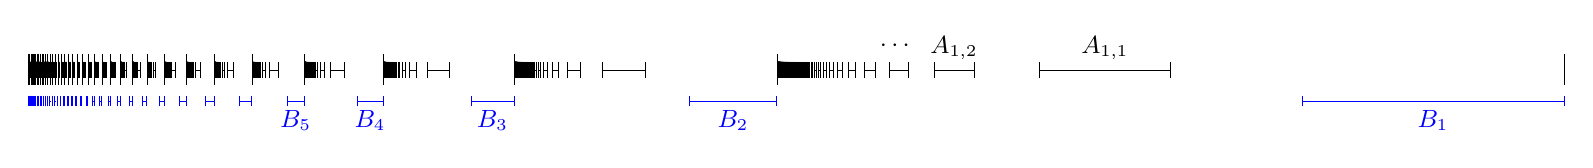
\begin{tikzpicture}[scale=2, xscale=10]
  \pgfmathsetmacro{\lheight}{.1}
  \foreach \n in {1, 2,..., 40}{
    \pgfmathsetmacro{\ax}{1/\n}
    \pgfmathsetmacro{\cn}{1/\n - 1/(\n + 1)}

    \draw[very thin] (\ax, \lheight) -- (\ax, -\lheight);

    \pgfmathsetmacro{\bna}{1/(\n + 1) + \cn*2/3}
    \pgfmathsetmacro{\bnb}{1/\n}

    \draw[blue, very thin, |-|] (\bna, -2*\lheight) -- (\bnb,
    -2*\lheight);

    \pgfmathsetmacro{\mmax}{500/\n}
    \foreach \m in {1, 2,..., \mmax}{
      \pgfmathsetmacro{\newax}{1/(\n+1) + \cn/(2*\m + 1)}
      \pgfmathsetmacro{\newbx}{1/(\n+1) + \cn/(2*\m)}

      \draw[ultra thin] (\newax, .5*\lheight) -- (\newax, -.5*\lheight);
      \draw[ultra thin] (\newbx, .5*\lheight) -- (\newbx, -.5*\lheight);
      % \draw[{Bracket[]-Bracket[]}, ultra thin] (\newax, 0) -- (\newbx, 0);
      \draw[ultra thin] (\newax, 0) -- (\newbx, 0);

      % \draw (\newax, 0) -- (\newbx,)
    }
  }

  \foreach \n in {1,2,3,4,5}{
    \pgfmathsetmacro{\cn}{1/\n - 1/(\n + 1)}

    \pgfmathsetmacro{\bna}{1/(\n + 1) + \cn*2/3}
    \pgfmathsetmacro{\bnb}{1/\n}

    \path (\bna, -2*\lheight) -- (\bnb, -2*\lheight) node[midway,
    below, blue] {\small $B_\n$};
  }

  \foreach \m in {1, 2}{
    \pgfmathsetmacro{\n}{1}
    \pgfmathsetmacro{\cn}{1/\n - 1/(\n + 1)}
    \pgfmathsetmacro{\newax}{1/(\n+1) + \cn/(2*\m + 1)}
    \pgfmathsetmacro{\newbx}{1/(\n+1) + \cn/(2*\m)}

    \path (\newax, 0) -- (\newbx, 0) node[above, midway] {\small $A_{\n,
        \m}$};

  }

  \node () at (.575, .15) {\small $\cdots$};


\end{tikzpicture}
\end{document}
